\documentclass[12pt]{spieman} 
\usepackage{amsmath,amsfonts,amssymb}
\usepackage{graphicx}
\usepackage{setspace}
\usepackage{tocloft}

\begin{document} 

\tableofcontents
\newpage
\section{Material from terrestrial measurement}
\subsection{Control points}
The points were taken from the measurement and interpretation of aerial
images, for the signalization of the control points crosses from the white PVC foil were used. Material from a terrestrial measurement was obtained by the tachymetric measurement in the area of the University Forest Enterprise.

Algorithms for image comparison can be used with automatic orientation  of aerial images, triangulation, manual, half-automatic, automatic digital terrain model generation. A digital photogrammetric system should include these modules:
\begin{itemize}
\item[-] Import of scanned aerial images and data from GIS/CAD; 
\item[-] Modification of the image radiometric attributes (filtering, contrast changing); 
\item[-] Mono and stereo image interpretation;
\item[-] DTM processing (automatic generation, displaying, editing); 
\item[-] Automatic modules (image comparison, image classification); 
\item[-] Image transformation (planar, ortho-photo generation). 
\end {itemize}

 Known algorithms have been implemented to solve the problems of classic photogrammetry such as triangulation (\ref{1}), aerial image orientation, orthoprojection, stereoscopic measurement.
 \begin{equation}
RMSE_{x}=\sqrt{\frac{1}{n}\sum\limits_{i=1}^n (E_{x,i})^2},\label{1}
  \end{equation}
  
  Transition from analogue to digital photogrammetry is inhibited the use of the other photogram- metric devices and all processing computers (\ref{2}). Digital photogrammetry includes some methods for image processing and computer vision, e.g. filtering, sharpening, contrast changing.
 \begin{equation}
  RMSE_{horizontal}=\sqrt{\frac{1}{m}\sum\limits_{i=1}^m |(E_{x,i})^2 +(E_{y,i})^2|}.\label{2}
 \end{equation}
 
  This paper proposes an approach to automatically extract LCPs from the LiDAR mobile mapping system (L-MMS) and UAV imagery used in the AT. The proposed strategy consists of three main steps as follows: 
\begin{enumerate}
\item  Generate image-based sparse point clouds via a SfM strategy; 
\item  Iterative plane fitting approach for extraction of LCPs from L-MMS; 
\item  Refine IOPs of a camera, EOPs of block images, and estimating OPCs of tie points through a BA procedure. 
\end{enumerate}

Here, it is assumed that L-MMS data as a reference spatial in- formation. In one hand, it is supposed that all EOPs and IOPs of image sensors are inaccurate and should be reliably estimated. These inaccurate EOPs and IOPs values are related to approximate sensor positions and non-metric camera parameters. On the other hand, not much attention has been paid to a handheld laser scanners used in L-MMS. In this study due to the above necessities, we investigate the benefits of extracting control points Figure \ref{f1}  from L-MMS data for being used in a photogrammetric UAV network. 
\begin{figure}[H] 
\centering{
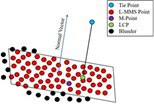
\includegraphics[width=50mm]{f1.jpg}
}
\caption{Representation of the tie point and its projection on the plane}
\label{f1}
\end{figure}

\subsection{Aerial image interpretation using the Imagestation ssK system}
 The system ImageStation SSK was used for the photogrammetric interpretation of aerial images and for their planimetry and elevation accuracy determination. The module ImageStation Stereo Display enabled their stereo displaying, coordinate readout, as well as bright and contrast correction in the case of the bad resolution of objects. Stereo glasses with the infrared emittor and pointing device were used for the interpretation, as well as stereo zoom, stereo displaying and movement over the stereo model (\ref{3}). Measured data were saved to a database. 
\begin{equation}
NCC=\frac{1}{\sqrt{\sum\limits_{i=1}^m\sum\limits_{j=1}^n(x_{i,j}-\overline{x})^2}\sqrt{\sum\limits_{i=1}^m\sum\limits_{j=1}^n(y_{i,j}-\overline{y})^2}}{\sum\limits_{i=1}^m\sum\limits_{j=1}^n(x_{i,j}-\overline{x})(y_{i,j}-\overline{y})}\label{3}
\end{equation}

For the infrared and black and white image pair the coordinates (X, Y, Z) were read out at 41 check points only once Table \ref{tab:table}. 
\begin{table}[H]
\caption{Results organized according to the number of control points used in the projects}
\centering
\begin{tabular}{|c|c|c|c|c|c|c|}
\hline
&\multicolumn{4}{c|}{Aerotriangulation accuracy} &\multicolumn{2}{c|}{Orthophoto accuracy} \\  
&\multicolumn{4}{c|}{} & \multicolumn{2}{c|}{$m_{xy}$} \\ 
\cline{2-7}
& $m_{x}$ & $m_{y}$ & $m_{z}$ & $m_{xy}$ & area N\textsuperscript{\underline{o}} 1 & area N\textsuperscript{\underline{o}} 2 \\
\hline
Project 1 & 0.2717 & 0.2429 & 0.6457 & 0.2577 & 0.9087 & 0.7008\\
\hline
Project 8 & 0.2015 & 0.1985 & 0.5103  & 0.2000 & – & – \\
\hline
Project 2 & 0.2908 & 0.2384 & 0.6417 & 0.2659 & 11.6960 & 0.9429 \\
\hline
Project 7 & 0.2103 & 0.2095 & 0.5522 & 0.2100 & – & –\\
\hline
Project 3 & 0.2516 & 0.2322 & 0.6803 & 0.2421 & – & 15.8450\\
\hline
Project 6 & 0.2167 & 0.2216 & 0.6032 & 0.2190 & – & –\\
\hline
Project 5 & 0.2733 & 0.2792 & 0.7072 & 0.2760 & – & – \\
\hline
Project 4 & 0.2125 & 0.2305 & 0.8227 & 0.2217 & 0.3545 & 0.8470 \\
\hline
DMT-auto. & – & – & – & – & 0.5664 & 0.7075 \\
\hline
DMT-man. & – & – & – & – & 0.4069 & 0.5494 \\
\hline
\end{tabular}
\label{tab:table}
\end{table}

\subsection {Digital aerotriangulation}
 After aerotriangulation ISAT automatically generates computed coordinates at the check points, so it is possible to statistically evaluate their accuracy. These check points are imported and edited with the control points, but with the check point attributes given (\ref{4}). They can also be used for densification or as detailed points.  
 \begin{equation}
S =
\begin{Vmatrix}
\begin{bmatrix}
x \\
y \\
z \\
\end{bmatrix} 
\end{Vmatrix}
+
\begin{Vmatrix}
\begin{bmatrix}
\Delta{x_R} \\
\Delta{y_R}  \\
\Delta{z_R} \\
\end{bmatrix} 
\end{Vmatrix}
\label{4}
\end{equation} 
where S – minimum score value in the compatibility analysis; 
x, y, z – vector coordinates. 

If there are no such points imported before, their coordinates can also be determined in the software product (ISSD), by measuring with the stereo cursor Figure \ref{f2}. The main working absolute and relative orientation was processed in the ImageStation Model Setup (ISMS), using 5 control points for each image pair (black and white, infrared). 
\begin{figure}[H] 
\centering{
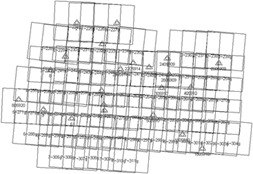
\includegraphics[width=50mm]{f2.jpg}
}
\caption{Distribution of the control points}
\label{f2}
\end{figure}

\end{document}